\documentclass[10pt]{exam}
\usepackage[icp]{template-for-exam}
\usepackage{circuitikz,multicol}


\title{Circuits Practice}
\author{Rohrbach}
\date{\today}

\begin{document}
\maketitle

\begin{questions}

\question
  Which of the following circuits will have more current?  How do you know?

  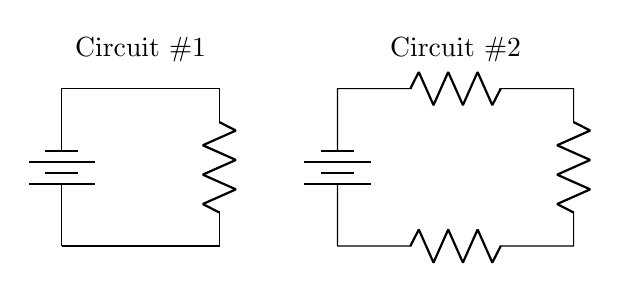
\begin{tikzpicture}
    \draw (0,0) 
      to[battery]  ++(0,2)
      to[short]    ++(2,0)
      to[resistor] ++(0,-2)
      to[short]    ++(-2,0);

    \draw (3.5,0) 
      to[battery]  ++(0,2)
      to[resistor] ++(3,0)
      to[resistor] ++(0,-2)
      to[resistor] ++(-3,0); 

    \node at (1,2.5) {Circuit \#1};
    \node at (5,2.5) {Circuit \#2};
  \end{tikzpicture}

\vspace{1em}
\hrule

\question
  Consider the following circuit. Before the switch is turned on, which lights are lit?

  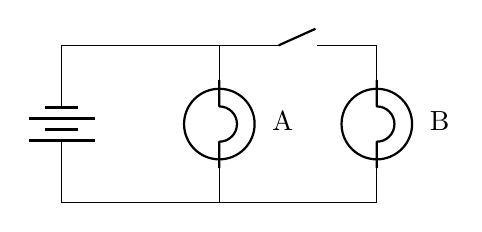
\begin{tikzpicture}
    \draw (0,0) 
      to[battery]  ++(0,2)
      to[short]    ++(2,0)
      to[bulb,l=A] ++(0,-2)
      to[short]    ++(-2,0);
    \draw (2,2) 
      to[normal open switch]  ++(2,0)
      to[bulb,l=B]            ++(0,-2)
      to[short]               ++(-2,0);
  \end{tikzpicture}

\vspace{1em}
\hrule

\question
  Consider the following circuit.  If bulb A breaks, which bulbs will remain lit?  Explain how you know.
  
  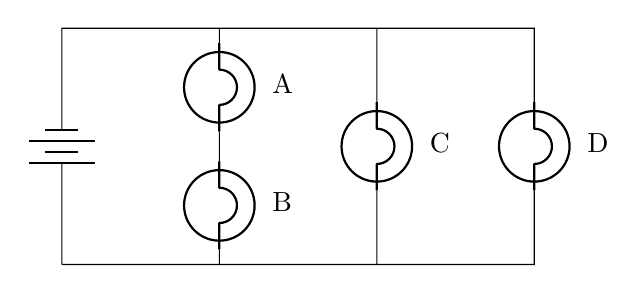
\begin{tikzpicture}
    \draw (0,0) 
      to[battery]  ++(0,3)
      to[short]    ++(2,0)
      to[bulb,l=A] ++(0,-1.5)
      to[bulb,l=B] ++(0,-1.5)
      to[short]    ++(-2,0);
    \draw (2,3) 
      to[short]    ++(2,0)
      to[bulb,l=C] ++(0,-3)
      to[short]    ++(-2,0);
    \draw (4,3) 
      to[short]    ++(2,0)
      to[bulb,l=D] ++(0,-3)
      to[short]    ++(-2,0);
  \end{tikzpicture}

\vspace{1em}
\hrule

\question
  Consider the following circuit.  If bulb D breaks, which bulbs will remain lit?  Explain how you know.
  
  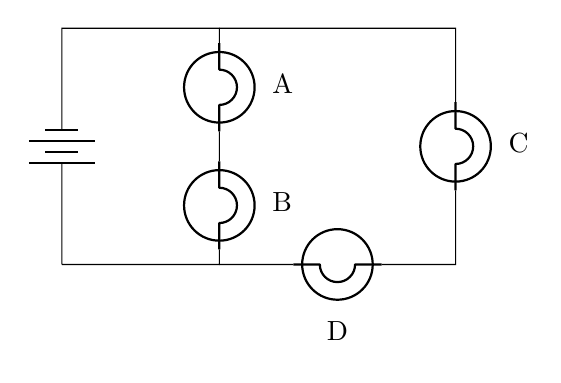
\begin{tikzpicture}
    \draw (0,0) 
      to[battery]  ++(0,3)
      to[short]    ++(2,0)
      to[bulb,l=A] ++(0,-1.5)
      to[bulb,l=B] ++(0,-1.5)
      to[short]    ++(-2,0);
    \draw (2,3) 
      to[short]    ++(3,0)
      to[bulb,l=C] ++(0,-3)
      to[bulb,l=D] ++(-3,0);
  \end{tikzpicture}

\hrule

\question
  Label each of the following types of circuits:

  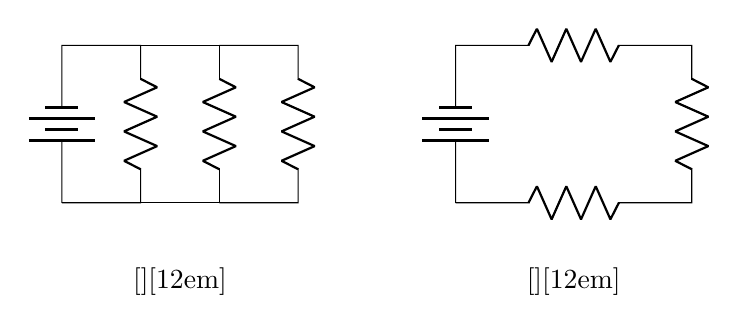
\begin{tikzpicture}
    \draw (0,0) 
      to[battery]  ++(0,2)
      to[short]    ++(1,0)
      to[resistor] ++(0,-2)
      to[short]    ++(-1,0);
    \draw (1,2) 
      to[short]    ++(1,0)
      to[resistor] ++(0,-2)
      to[short]    ++(-1,0);
    \draw (2,2) 
      to[short]    ++(1,0)
      to[resistor] ++(0,-2)
      to[short]    ++(-1,0);

    \draw (5,0) 
      to[battery]  ++(0,2)
      to[resistor] ++(3,0)
      to[resistor] ++(0,-2)
      to[resistor] ++(-3,0); 
      
    \node at (1.5,-1) {\fillin[][12em]};
    \node at (6.5,-1) {\fillin[][12em]};

  \end{tikzpicture}
  
\pagebreak

\question
  When you remove one light from a strand of Christmas lights, all of the other lights go out.  What kind of a circuit is the strand of Christmas lights?
  \vspace{5em}

\question
  Is your house wired as a series circuit or parallel circuit? How can you tell?
  \vspace{5em}

\question
  Fill in the missing charges.

  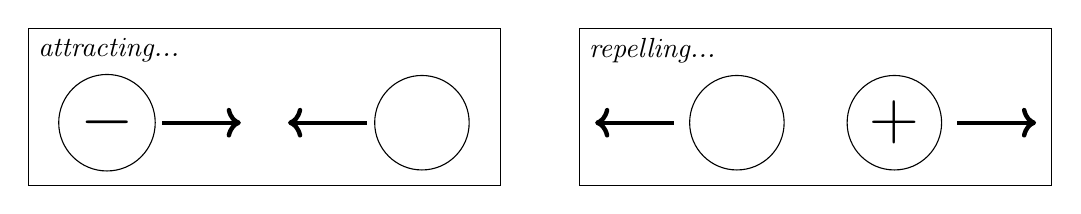
\begin{tikzpicture}
    \begin{scope}
      \node[anchor=north west] at (0,2) {\emph{attracting...}};
      \draw (0,0) rectangle (6,2);
      \node[circle,minimum size=1.2cm,draw=black] 
        at (1,.8) {\Huge $-$};
      \node[circle,minimum size=1.2cm,draw=black] 
        at (5,.8) {};
      \draw[->,ultra thick] (1.7,.8) -- ++(1,0);
      \draw[->,ultra thick] (4.3,.8) -- ++(-1,0);
    \end{scope}

    \begin{scope}[shift={(7,0)}]
      \node[anchor=north west] at (0,2) {\emph{repelling...}};
      \draw (0,0) rectangle (6,2);
      \node[circle,minimum size=1.2cm,draw=black] 
        at (2,.8) {};
      \node[circle,minimum size=1.2cm,draw=black] 
        at (4,.8) {\Huge $+$};
      \draw[->,ultra thick] (1.2,.8) -- ++(-1,0);
      \draw[->,ultra thick] (4.8,.8) -- ++(1,0);
    \end{scope}
  \end{tikzpicture}


\question
  A 1.5-volt battery is hooked up to a 10-ohm resistor.  What is the current?
  \ku[3cm]

\question
  What is the voltage through a circuit that has a current of 0.5 amps and a resistance of 30 ohms?
  \ku[3cm]

\question
  What is the current through the following circuit?
  
  \begin{tikzpicture}
    \draw (0,0) 
      to[battery ,l=\SI{ 3}{\volt}] (0,2)
      to[resistor,l=\SI{30}{\ohm}]  (3,2)
      to[resistor,l=\SI{10}{\ohm}]  (3,0)
      to[short]                     (0,0);

    \node[anchor=north west] at (4,3) 
      {Knowns/Unknowns};
    \node[anchor=north west] at (7.6,3)
      {Plug \& Chug};
    \node[anchor=north west] at (11.8,3) 
      {Answer w/ Units};
    \draw (7.4,3) -- ++(0,-4);
    \draw (11.6,3) -- ++(0,-4);

  \end{tikzpicture}


  

    
\end{questions}

\end{document}